%*****************************************
\chapter{Stand der Forschung}\label{ch:relatedWork}
%*****************************************

\section{Die Ontologie: SNIK}

Das semantische Netz des Informationsmanagements im Krankenhaus (\ac{snik}) ist eine am \ac{imise} der Universität Leipzig entwickelte,
die Domäne des Informationsmanagements im Krankenhaus betreffende Ontologie \citep{domaene}.
Sie behandelt Wissen über Krankenhausinformationssysteme und deren Management.
Dieses wurde aus drei Lehrbüchern (\citet{bb}, \citet{ob} und \citet{he}) manuell extrahiert und in RDF modelliert.
Desweiteren wurde auch noch ein Interview mit dem Leiter des Informationsmanagements des Universitätsklinkum Leipzigs, Stefan Smers, geführt.

\begin{sidewaysfigure}[htbp!]
\centering
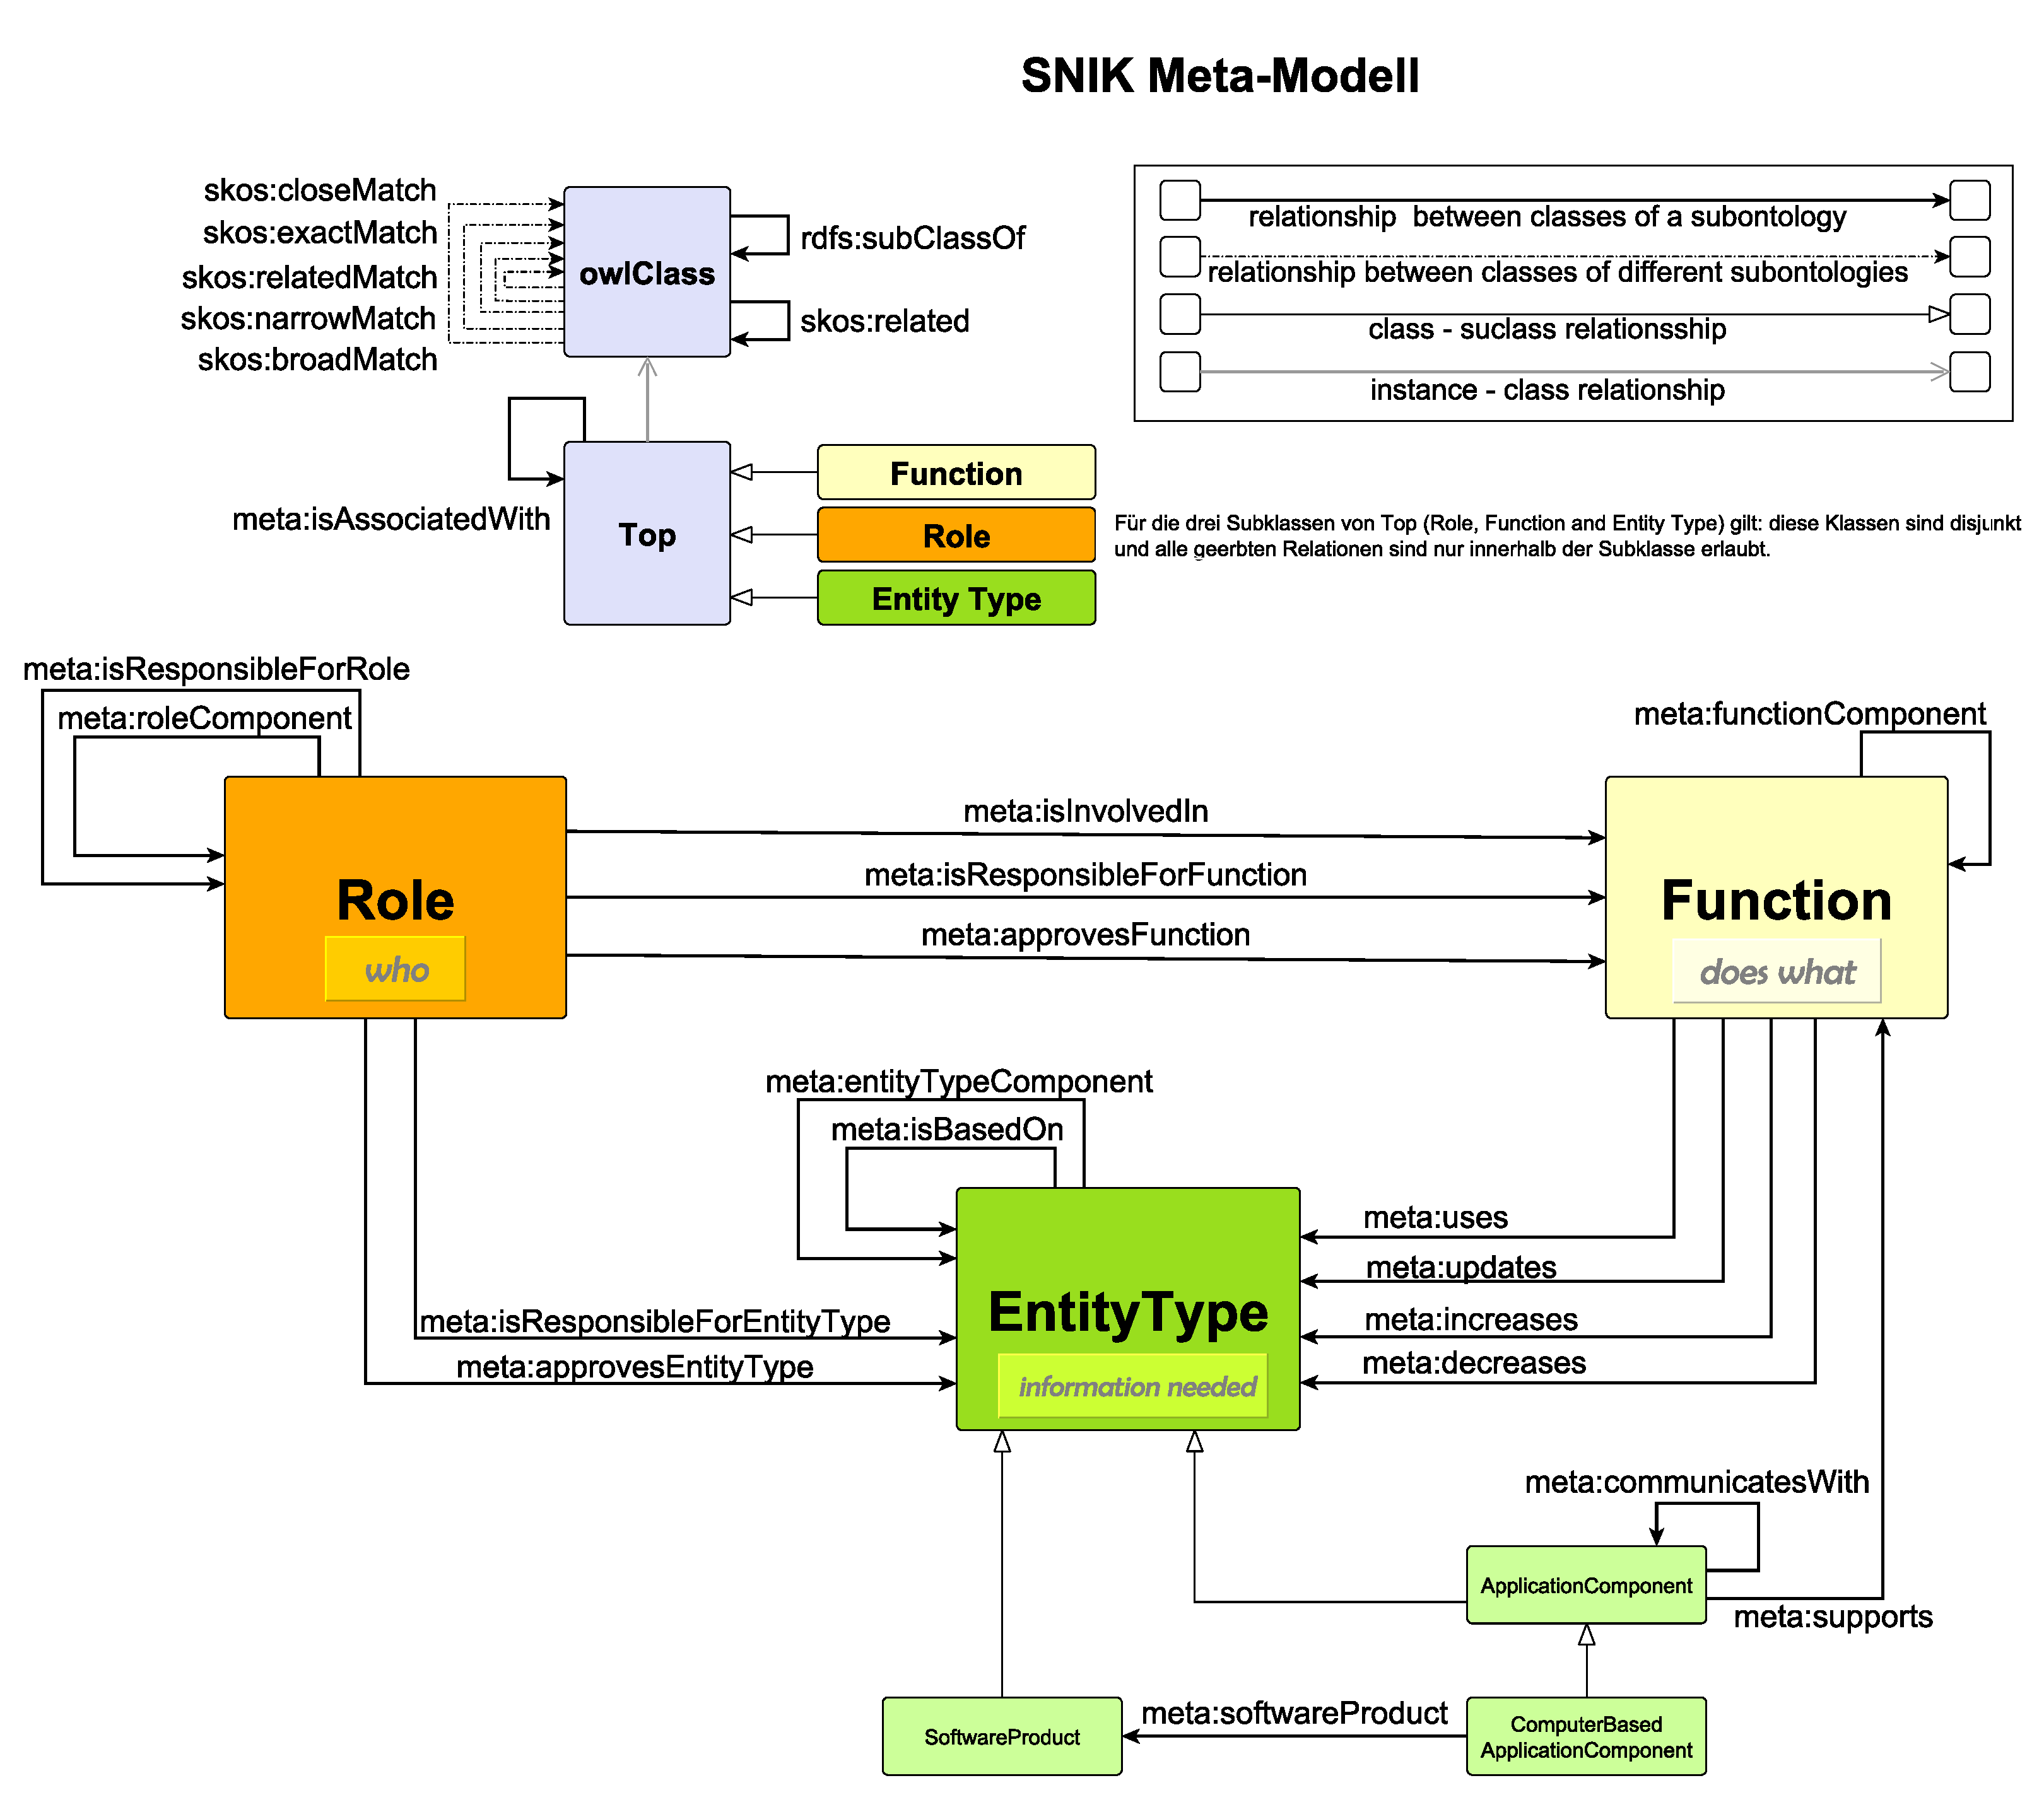
\includegraphics[width=.8\textwidth, height=.9\textheight, keepaspectratio]{Images/snik-metamodel.pdf}
\caption[SNIK Metamodell Version 8]{Das SNIK Metamodell Version 8. Quelle: \url{https://www.snik.eu/public/SNIK_Metamodell_V8.svg}}
\label{fig:snik-metamodel}
\end{sidewaysfigure}

\subsection{\enquote{Eine Ontologie von Ontologien} - Die Architektur SNIKs}

Die einzelnen Bücher liegen jeweils in einer eigenen Subontologie vor.
Es gibt also drei große Teilontologien der \ac{snik}-Ontologie, die die Präfixe \emph{bb}, \emph{ob} und \emph{he} haben.
Das Interview mit dem Leiter des Informationsmanagements befindet sich in der Subontologie mit dem Präfix \emph{ciox}.
Zur Beschreibung der Relationen gibt es eine Ontologie mit dem Präfix \emph{meta}, in der größtenteils Properties stehen.
Diese enthalten dann jeweils Klassen von Individuen, z.B. \aurl{bb}{ChiefInformationOfficer} anstelle von \aurl{ex}{ErikaMustermann}.
Es geht hier nämlich, wie gesagt, um Textbuchwissen und nicht um spezielle Vorgänge \ac{sniktec}.

Die Entitäten\ac{snik}s in einer Subontologie sind, wie in \cref{fig:snik-metamodel} zu sehen, primär nach ihrem Typ gegliedert.
Es gibt Rollen, die eine Person einnehmen kann, wie z.B. \aurl{bb}{ChiefInformationOfficer}, Aufgaben, die eine Rolle hat, wie z.B. \aurl{bb}{HISBudgetPlanning},
und Objekttypen, die Informationen, die für diese Aufgabe benötigt werden, repräsentieren, wie z.B. \aurl{bb}{AnnualITBudget}.
Zwischen diesen gibt es Relationen, die deren Beziehung beschreiben.

Die Subontologien sind theoretisch unabhängig voneinander. Sie sind größtenteils dann verbunden,
wenn sie ähnliche Prinzipien wie ein anderer Punkt einer anderen Subontologie darstellen.
Für das Tripel mit dem Subjekt \aurl{bb}{ChiefInformationOfficer} gibt es das Prädikat \aurl{skos}{closeMatch} mit dem Objekt \aurl{ciox}{ChiefInformationOfficer}.
Es gibt dieses Tripel auch mit diesem als Subjekt und dem anderen als Objekt.
Dies erklärt auch, weshalb auf dem Pfeil zwischen ihnen keine Richtung zu sehen ist.


\subsection{Der SNIK-Graph}

Der \ac{snik}-Graph\footnote{\url{https://www.snik.eu/graph}} ist die Visualisierung von \ac{snik}.
Hier werden die einzelnen Entitäten nach ihrer entsprechenden Subontologie gefärbt visuell dargestellt.
Die beschrifteten Verbindungen bzw. Kanten zwischen den Formen stellen Relationen dar,
welche, wenn sie zwischen zwei Entitäten unterschiedlicher Subontologien verlaufen, keine Richtung haben.
Entitäten werden durch Dreiecke, Quadrate oder Kreise dargestellt und vertreten die verschiedenen Typen.

\section{Stichwortsuche}

Die Stichwortsuche ist wohl mit die am weitesten verbreitete Form, um sich Informationen anzueignen.
Im Gegensatz zu Question Answering werden hier statt ganzen Sätzen nur einzelne Stichwörter eingegeben, womit letztendlich Ergebnisse angezeigt werden.
Das Problem (bzw. der Ansatz) dabei ist nicht unbedingt, den Nutzer zu verstehen, sondern in abertausenden Möglichkeiten die möglichst relevantesten herauszusuchen.
Dazu werden oft Listen, wo die Antwortmöglichkeiten indiziert sind, verwendet.
Stichwortsuche wird nicht nur im \ac{www}, sondern auch in vielen anderen Bereichen eingesetzt.
Manche Question Answering-Systeme verwenden es z.B. auch für bestimmte Module.

\subsection{Elasticsearch}

Elasticsearch\footnote{\url{https://www.elastic.co}} ist ein Open-Source Programm, das einfaches Indizieren, Suchen und Analysieren von Daten ermöglichen soll \citep[S.~8]{elasticsearch}.
Es kann verschiedenste Datentypen durchsuchen, auch Text und Zahlen.
Dazu serialisiert es Dokumente in \ac{json}, einer für die Programmiersprache JavaScript, welche häufig auf Webseiten verwendet wird, lesbare Notation.
In dieser Serialisierung nutzt es einen \emph{invertierten Index}, d.h. es indiziert das Dokument für alle verschieden vorkommenden Wörter \citep{invertedindex}.
Das Wort bzw. die Zeichenkette ist also ein Schlüssel mit den Dokumenten als Wert.
Nehme man z.B. die beiden Sätze \enquote{War is peace.} und \enquote{Freedom is slavery.}\todo{Orwell zitieren/Beispiel aus SNIK} als eigene Dokumente, würde es wie in \cref{tab:invertedindexexample} aussehen.
Das Wort \enquote{is} kommt sowohl in Dokument 1 und 2, das Wort \enquote{war} nur in Satz 1 und das Wort \enquote{freedom} in nur in Satz 2.
Die Zahl nach dem Doppelpunkt zeigt die Position im Satz an, \enquote{peace} ist z.B. an dritter Stelle im ersten Satz.
\begin{table}[h]\centering
  \begin{tabulary}{\textwidth}{rl}
    \toprule
    Schlüssel & Wert(e) \\
    \midrule
    war & 1:1 \\
    is & 1:2,2:2 \\
    peace & 1:3 \\
    freedom & 2:1 \\
    slavery & 2:3 \\
    \bottomrule
  \end{tabulary}
  \caption{Beispiel für invertierte Indizes}
  \label{tab:invertedindexexample}
\end{table}
Elasticsearch verwendet \ac{rest}-\acp{api}, also Programmierschnittstellen, die mittels \ac{http}-Anfragen mit Seiten im \ac{xml}-Format, wie z.B. \ac{html}, kommunizieren.
Mit diesen kann es in der Tabelle nach Informationen suchen.
Das tut es, indem es die Seiten und Positionen, auf denen die eingegebenen Wörter stehen, mithilfe der invertierten Indizes heraussucht.
Je näher die eingegebenen Wörter aneinanderstehen, und je eher die gefundenen Wörter mit den eingegebenen übereinstimmen, desto besser ist das Ergebnis und desto eher wird es angezeigt.
Es können auch verschiedene Synonyme und phonetisch ähnlich klingende Wörter ausprobiert werden.

\section{Question Answering-Systeme}

Zur Recherche wurden verschiedene Surveys bezüglich \ac{kbqa} bzw. \ac{cdqa} verwendet.
Außerdem wurde über die Herausforderung \ac{qald}, wo mithilfe eines Fragenkatalogs versucht wird, Question Answering-Systeme objektiv zu bewerten.
Als Trainingssatz wird DBpedia verwendet \citep{qald9}.

DBpedia ist eine Ontologie, die aus den Daten Wikipedias besteht.
Es ist das Paradebeispiel für Linked Data und wird häufig zum Training von Question Answering-Programmen genutzt.
Die Daten sind frei und in verschiedenen Formaten, wie z.B. als \ac{rdf}-Tripel, verfügbar.
Über \ac{sparql} können auch direkt online Abfragen getätigt werden.
DBpedia ist außerdem in mehreren Sprachen verfügbar \citep{dbpedia}.

\subsection{Leaderboard}

Das Question Answering-Leaderboard\footnote{\url{https://github.com/KGQA/leaderboard}} \citep{kgqaleaderboard} hat es sich zur Aufgabe gemacht,
das häufig als sehr uneinheitlich \citep{diefenbachkbqa} beschriebene Feld des \ac{kbqa}\todo{Leaderboard}

\subsection{gAnswer}

gAnswer\footnote{\url{https://github.com/pkumod/gAnswer}} \citep{ganswer2} wurde von dem Wangxuan Institute of Computer Technology entwickelt und arbeitet mit Wissensbasen, um Question Answering-Aufgaben zu lösen.
Hierfür werden die Fragen in Unterfragen aufgespalten und daraus je ein Syntaxbaum erstellt.
Es erzielte durch eine durchdachte Vorbereitung der Trainingsdaten sehr schnelle Trainingszeiten bei niedrigem Speicherverbrauch und hoher Genauigkeit bei der Beantwortung von Fragen.
Das System hat außerdem die Umformung von natürlicher Sprache in \ac{sparql}-Abfragen als das Problem,\todo{besser erklären, nochmal drüberschauen bzw. Satz entwirren}
Subgraphen zu vergleichen, erkannt, und somit einen neuen Ansatz zur Lösung des Problems der Homonymität geboten.
Das bedeutet, dass Wörter, die Verschiedenes bedeuten können, erst nach anfänglicher Lokalisierung des Kontexts betrachtet werden.
Es werden also zuerst Wörter, deren Bedeutung eindeutig ist, betrachtet, und von da aus die kürzeste Verbindung zu einer Bedeutung des fragwürdigen Wortes \citep{ganswerapproach}.
Darauf bauen viele andere Question Answering-Systeme auf.

\subsection{DeepPavlov}
DeepPavlov\footnote{\url{https://www.deeppavlov.ai}} \citep{deeppavlov} ist eine open-source Bibliothek zur Entwicklung von Dialogsystemen.
Es ist in \emph{Models} und \emph{Skills} organisiert.
Das System ist hochdynamisch und auf verschiedenste Aufgaben ausgelegt, vor allem aber Dialogsysteme bzw. Chat Bots.
Für Question Answering gibt es bisher nur Ansätze bezüglich \ac{odqa}.

\subsubsection{Architektur}
Ein \emph{Model} ist eine in TensorFlow \citep{tensorflow}, einer Schnittstelle für maschinelles Lernen, implementierte Funktion einer \ac{nlp}-Pipeline,
die sowohl ein neuronales Netz als auch ein nichtneuronales oder regelbasiertes System sein kann.
Models können auch andere Models enthalten.
Ein \emph{Skill} besteht aus Models, jedoch kann er nur Zeichenketten als Ein-/Ausgabe haben.
Sie werden deshalb häufig im Dialog verwendet.
Die Models in Skills werden über einen \emph{Chainer} verbunden, der die Konfigurationsdatei einliest und so die Parameter der Models festsetzt.
Skills und Models werden gleich implementiert und unterscheiden sich nur in den Unterschiedlichen Ein- und Ausgabemöglichkeiten.
Mehrere Skills formen einen \emph{Agent}, wie in \cref{fig:deeppavlov-architektur} sichtbar ist.
Ein Agent kann die verschiedenen Skills, aus denen er besteht, in einer Unterhaltung mit dem Benutzer verwenden und zwischen ihnen wechseln.

\begin{figure}[htbp!]
\centering
\includegraphics[width=\textwidth, height=\textheight, keepaspectratio]{Images/DeepPavlovArchitecture.png}
\caption[DeepPavlov Architektur]{Die Architektur von DeepPavlov. Quelle: \citet{deeppavlov}}
\label{fig:deeppavlov-architektur}
\end{figure}

\subsection{TeBaQA}

TeBaQA\footnote{\url{https://github.com/dice-group/TeBaQA}} \citep{tebaqa} wird von der Forschungsgruppe DICE an der Universität Paderborn entwickelt.
Es basiert darauf, Fragen anhand ihrer Struktur zu gruppieren.
Dabei werden isomorphe \ac{sparql}-Anfragen, d.h. Anfragen gleicher Struktur, einer Vorlage zugeordnet.
Somit können schnellere Antwortzeiten ermöglicht werden.
Mit Struktur ist die Form der RDF-Relationen gemeint, wobei diese als Kanten zwischen den verschiedenen Informationen gesehen werden.

\subsubsection{Architektur}

TeBaQA wird in fünf Phasen aufgebaut.
In der ersten Phase, dem \emph{Preprocessing} (Vorverarbeitung), werden Wörter, die keinen semantischen Wert und somit keine Information tragen, entfernt.
Das können etwa Artikel sein, wodurch die Assoziation der Wörter mit vielen unzusammenhängenden Einträgen vermieden wird.
Damit solche Wörter, die auch Teil der Entitäten, wie z.B. \enquote{the} in \aurl{bb}{AdaptabilityOfTheHIS},
nicht auch dort herausgefiltert werden, müssen die Wörter gruppiert und die resultierenden Gruppen überprüft werden.
Die zweite Phase befasst sich mit der Isomorphie der Abfragegraphen und der Vorlagenklassifizierung.
Hier wird die zu nutzende Vorlage der Abfrage identifiziert und darüber Eigenschaften der Frage, also z.B. Fragewörter,
Anzahl der Nomen, mindestens benötigte Tripel oder ob Personen referenziert werden.
Die Einordnung in eine Vorlage geschieht, wie vorher schon erwähnt, über die Struktur der \ac{sparql}-Abfrage.
Die Reihenfolge der Elemente wird hierbei nicht betrachtet.
Beispielsweise resultiert die Frage \enquote{Wofür ist die Leiterin des Informationsmanagements zuständig?}
in einer Abfrage mit der gleichen Struktur wie die Abfrage der Frage \enquote{Wovon wird 3LGM² erzeigt?}.
Die \ac{sparql}-Abfrage könnte bei beiden so aussehen, bei der ersten Abfrage wäre das Individuum im Subjekt \aurl{bb}{ChiefInformationOfficer} und das Prädikat \aurl{meta}{isResponsibleForEntityType},
bei der zweiten Frage das Subjekt \aurl{bb}{3LGM2} und das Prädikat \aurl{meta}{isBasedOn}.
\begin{lstlisting}
  PREFIX bb: <http://snik.eu/ontology/bb/>
  PREFIX meta: <http://snik.eu/ontology/meta/>
  SELECT ?uri
  WHERE
    { <Subjekt> <Prädikat> ?uri }
\end{lstlisting}
Das Ergebnis, ?uri, ist \aurl{bb}{AnnualITBudget} bzw. \aurl{bb}{UmlClassDiagram}, also beide Male eine Entität.
Wenn die Vorlage zugeordnet wurde, können Eigenschaften der Frage, wie oben beschrieben, in einen Vektor getan und weiterverwendet werden.
Im dritten Schritt werden speziell referenzierte Individuen und Klassen identifiziert, also nicht nur wie im 2. Schritt generelle Informationen über den Inhalt der Frage.
Hier werden auch verschiedene Synonyme der eingegebenen Wörter untersucht, um ein möglichst genaues Ergebnis zu erreichen.
Im vierten Schritt wird die Anfrage geschrieben, also die Vorlage gefüllt und eventuelle Parameter gesetzt.
Die letzte Phase behandelt das Auswählen der Lösung, die dem Nutzer übergeben werden soll.
Dazu wird wieder auf das Fragewort geblickt, um herauszufinden, in was für einer Form, z.B. einem Datum, der Nutzer die Antwort erwartet.
Das erste Substantiv nach dem Fragewort wird überprüft, um den Numerus der Frage zu erkennen.
Desweiteren werden die Lösungskandidaten auf ihre Ähnlichkeit mit der Frage überprüft, woraus eine Bewertung und letztendlich die zu präsentierende Antwort berechnet wird.
